% Chapter 4

\chapter{Implementation} % Main chapter title

\label{Chapter4} % For referencing the chapter elsewhere, use \ref{Chapter1} 

\lhead{Chapter 4. \emph{Implementation}} % This is for the header on each page - perhaps a shortened title

%----------------------------------------------------------------------------------------

% \emph{Diskuter de viktigste algoritmene og datastrukturene, og hvordan de utviklet seg, fremhev noen nye/originale funksjoner. Også diskuter hvordan du har tenkt å utføre testen din (validering og evaluering).}

This chapter will go through the algorithms and API calls being used by the application.

In addition to the three steps in chapter~\ref{Chapter3} -- ``data gathering'', ``sentiment analysis'', and ``rating prediction'' -- this chapter will also touch upon how the evaluation mechanisms were implemented. However, evaluation results and related discussions are deferred to chapter~\ref{Chapter5}.

\section{Languages and tools} % (fold)
\label{sec:languages_and_tools}

The system was implemented in the Python programming language, and has no further technical requirements. However, it supports using SQLite\footnote{\url{http://www.sqlite.org/}} to store and query various movie metadata, and to cache content classifications to avoid hitting the remote APIs too much during testing.

The final application is a highly configurable command-line tool. Its interface co-evolved with its requirements, and lets the user control most of its parameters. Figure~\ref{fig:tool_help} shows the result of running the final program with the \verb+--help+ argument.

\begin{figure}[h]
  \centering
    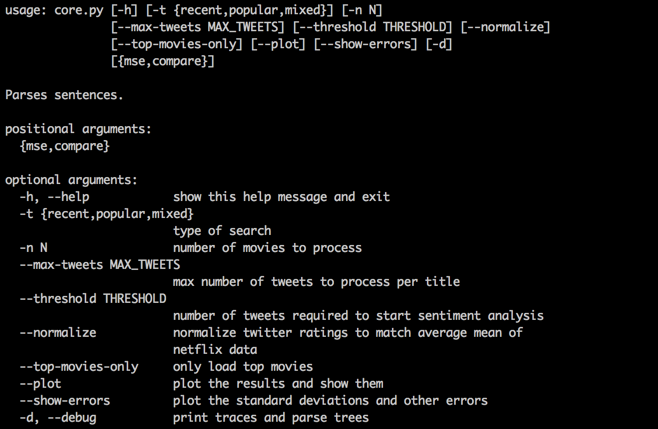
\includegraphics[width=.9\textwidth]{Figures/tool_help}
  \caption{Screenshot of the application's help menu.}
  \label{fig:tool_help}
\end{figure}

\subsection{Important data structures} % (fold)
\label{sub:data_structures}

The only somewhat complex entity being processed by the system is the Twitter messages. These are represented in the system as instances a simple \verb+Tweet+ class. It has a small set of default values and utility methods, but in practice, the objects behave as dictionaries.

Each \verb+Tweet+ object is augmented with additional metadata on its way through the system, until the ``rating predicion'' step, where they are reduced to real-numbered predictions and discarded.

\section{Data gathering} % (fold)
\label{sec:data_gathering_impl}

As was soon found out after the initial tinkerings with the Twitter API began, the service has a high noise ratio. An example of this is the search results depicted in figure~\ref{fig:search_simple}. A simple search for the movie title ``The Usual Suspects'' returns only noisy results -- none of them express any sort of sentiment about the actual movie.

\begin{figure}[h]
  \centering
    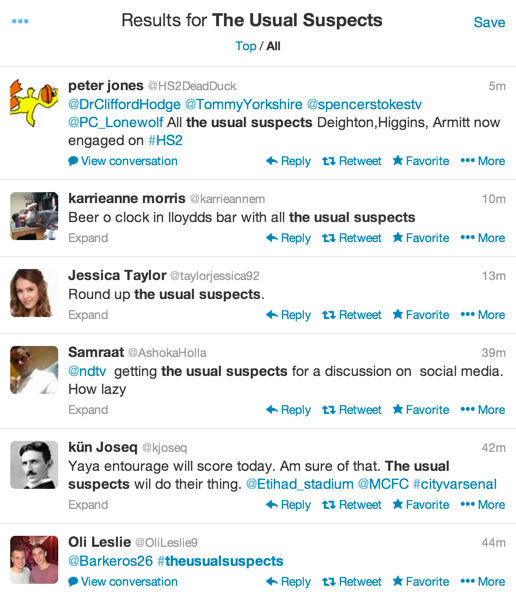
\includegraphics{Figures/search_simple}
  \caption{A simple search for ``The Usual Suspects'' gives only noisy results.}
  \label{fig:search_simple}
\end{figure}

Due to this noisiness, every opportunity was taken to refine and tweak the search queries used to gather content. Luckily, the Twitter API has a quite extensive search interface, with many ways of tweaking the results (details in section~\ref{ssec:search_api}).

After much trial and failure, the following settings seem to yield good results for typical well-known movies:

\begin{description}
  \item[Title as exact phrase] \hfill \\
    Ensure that the title is searched for in its entirety, as a singular phrase and not just the individual words. In the Twitter API this is done by enclosing the title in quotation marks, as such: \texttt{"The Usual Suspects"}, instead of \verb|The Usual Suspects|.
  \item[Exclude noisy terms] \hfill \\
    Exclude tweets containing the following terms\footnote{Any time a set of irrelevant results shared a common term, it would be added to the list. There are probably many ways of fine-tuning this further.}: \texttt{download}, \texttt{stream}, \texttt{\#nw}, \texttt{\#nowwatching}, and \texttt{RT}.
  \item[Add domain keyword as term] \hfill \\
    Some movies with a degree of cult status, such as ``The Usual Suspects''\footnote{\url{http://www.imdb.com/title/tt0114814/}}, can inspire usage of their titles as expressions in other contexts. This can lead to noisy results when they are used without referring to the movie. Some examples of this can be seen in figure~\ref{fig:search_simple_filtered}. Adding the domain term \texttt{movie} to the query rids us of many of these, as shown in figure~\ref{fig:search_filtered}. As we will see later, this still does not suffice for a lot of less-known movies.
\end{description}

\begin{figure}[h]
  \centering
    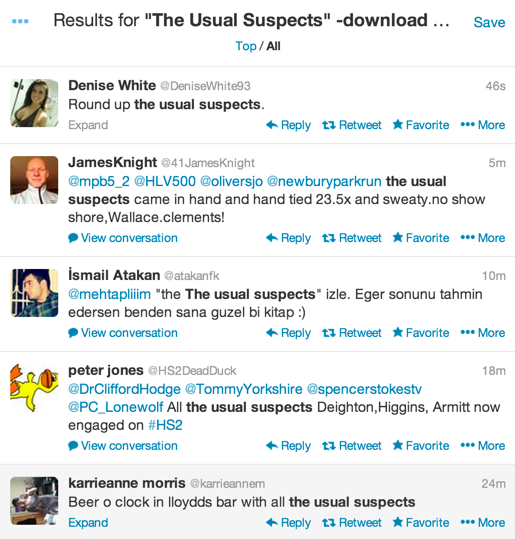
\includegraphics{Figures/search_simple_filtered}
  \caption{Without a domain term, many queries still return a lot of noise. This is the result of searching for \texttt{"The Usual Suspects" movie -download -stream -\#nw -\#nowwatching -RT}.}
  \label{fig:search_simple_filtered}
\end{figure}

\begin{figure}[h]
  \centering
    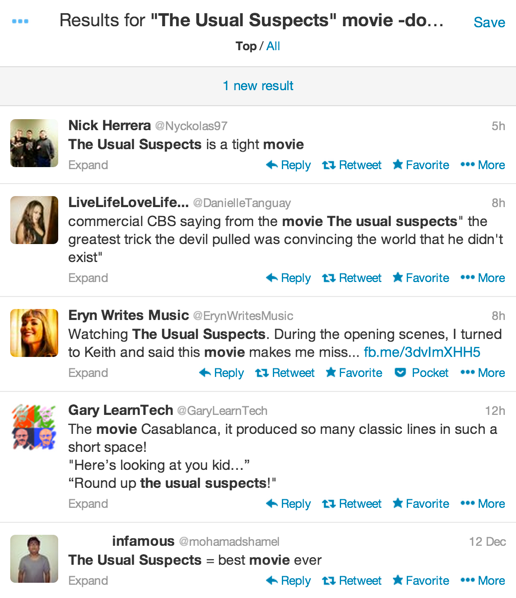
\includegraphics{Figures/search_filtered}
  \caption{The results of searching for \texttt{"The Usual Suspects" movie -download -stream -\#nw -\#nowwatching -RT}. A lot of noise has been eliminated, and most results are about the movie in questions.}
  \label{fig:search_filtered}
\end{figure}

For the choice among the three modes of search -- ``popular'', ``recent'', or ``mixed'' -- as much diversity as possible was desired. Although popular Tweets were initially preferred, there were simply not enough of them to warrant this choice (more often than not, zero or one). Therefore, to enable a fair comparison between popular and not-so-popular movie titles, the result type of choice became ``mixed''.

% section data_retrieval (end)

\section{Sentiment analysis} % (fold)
\label{sec:sentiment_analysis_impl}

A central part of the system is the sentiment classification of the Twitter results. This sentiment analysis could well have been implemented locally, but for simplicity's sake it has been offloaded to an external service called DatumBox\footnote{\url{datumbox.com}}, as it seems to employ a reasonable choice of algorithm, and performs well enough for our needs.

This section will take an in-depth look at the techniques the DatumBox service utilizes.

To get us started, this is how DatumBox themselves describe their classifier~\cite{DatumBoxTwitterSentiment}:

\begin{quote}
  In order to detect the Sentiment of the tweets we used our Machine Learning framework to build a classifier capable of detecting Positive, Negative and Neutral tweets. Our training set consisted of 1.2 million tweets evenly distributed across the 3 categories. We tokenized the tweets by extracting their bigrams and by taking into account the URLs, the hash tags, the usernames and the emoticons.

  In order to select the best features we used several different algorithms and at the end we chose the Mutual Information. Finally after performing several tests with various models and configurations we selected the Binarized Naïve Bayes as the best performing classifier for the particular problem (strangely enough Naïve Bayes beat SVM, Max Entropy and other classifiers which are known to perform usually better than NB). To evaluate the results we used the 10-fold cross-validation method and our best performing classifier achieves an accuracy of 83.26\%.
\end{quote}

There exists work which supports this results, where Naive Bayes outperforms SVM and Max Entropy in classifying Twitter messages~\cite{go2009twitter}.

The next sections will in turn describe feature selection by Mutual Information, and the Naive Bayes classifier.

\subsection{Feature selection by Mutual Information} % (fold)
\label{sub:feature_selection_by_mutual_information}

When selecting features one needs need a selection criteria. Typical approaches include Max-Dependency, Max-Relevance, and Min-Redundancy~\cite{1453511}. As an example, we'll have a quick look at the Max-Relevance scheme.

Max-Relevance involves choosing the features with the highest relevance to the target class $c$, and we typically characterize the concept of relevance in terms of mutual information. The mutual information of two random, discrete variables $X$ and $Y$ is given by~\eqref{eq:mutual_information}.

\begin{equation}
  I(X; Y) = \sum_{x \in X} \sum_{y \in Y} P(x, y) \log \frac{P(x, y)}{P(x) P(y)}
  \label{eq:mutual_information}
\end{equation}

Given a feature vector $f$ of length $n$, we want its $m$ most relevant features with respect to class $c$. The relevance of each feature $f_i$ is measured in order of its mutual information with the class $c$, ie. $I(f_i; c)$.

Thus, to extract the $m$ most relevant features with regard to class $c$, we simply order them in descending order by their $I(f_i; c)$, and keep the first $m$ elements.

% subsection feature_selection_by_mutual_information (end)

\subsection{The Naive Bayes classifier}
\label{ssec:nb_classifier}

To describe the Naive Bayes classifier we will use the bag-of-features framework~\cite{pang2002thumbs}.

Let ${f_1, f_2, \dotsc, f_m}$ be a set of $m$ features, and let $n_i(d)$ be the number of times $f_i$ occurs in document $d$. We can then represent each document $d$ as a vector $\vec{d} = (n_1(d), n_2(d), \dotsc, n_m(d))$. The training data being ``evenly distributed across the 3 categories''~\cite{DatumBoxTwitterSentiment}, the probability distribution $P(C)$ over the possible categories, $C$, is constant. We can therefore use the Maximum Likelihood approach to build our hypothesis, and simplify our calculations.

First, Bayes' rule tells us that

\begin{equation}
  P(c | d) = \frac{P(c) P(d | c)}{P(d)}
\end{equation}

where neither $P(d)$ nor $P(c)$ play any role in predicting $c$.

By assuming that the features $f_i$ are conditionally independent given their classes, we can formulate a maximum likelihood hypothesis which can be used to classify documents:

\begin{equation}
  h_{\text{ML}}(d) = \argmax_{c \in C} \prod_{i=1}^m P(f_i | c)^{n_i(d)}
\end{equation}

\subsection{Other issues}

When calling the DatumBox API, the best results were achieved when removing the movie title itself from the query. Quite a lot of titles have sentiment-carrying words in their titles\footnote{``Breaking Bad'' consequently scoring way below ``Cheers'' was a rather clear cut case.}, and this obviously confused the classifier quite a bit.

% section sentiment_analysis (end)


\section{Rating prediction} % (fold)
\label{sec:rating_prediction}

For rating prediction, the goal is to convert a set of sentiments into a single real number. The test set from Netflix uses integers from 1 to 5 inclusive, so the number should be within that range.

A simple linear solution was implemented, where a single sentiment $s$ is mapped into a real rating $r$ in the following way:

\begin{align*}
  r(\text{Positive}) &\rightarrow 5 \\
  r(\text{Neutral})  &\rightarrow 3 \\
  r(\text{Negative}) &\rightarrow 1
\end{align*}

The predicted rating $\hat{r}$ of a set of sentiments $S$ of size $n$ is defined as the mean of its individual sentiment values:

\begin{equation}
  \hat{r}(S) = \frac{1}{n} \sum_{s \in S} r(s)
\end{equation}

% section rating_prediction (end)

\section{Implementation of evaluation system} % (fold)
\label{sec:evaluation_impl}

To be able to consistently map the predictions back to the test set, the sample movies are drawn from the test set's own database. This set is comprised of a little over 17 thousand movies, and the only metadata available -- apart from the title -- is the year of release.

However, it soon became interesting to examine the difference in performance for popular and less-popular movies, and the system thus needed the ability to make this distinction. Therefore, IMDB's top 250 movies\footnote{\url{http://www.imdb.com/chart/top}} were dumped to a CSV file, and the 174 movies that matched ones in the evaluation set were marked as popular. This enabled the system to optionally restrict the drawn test sample to only those present in this list.

Although the movies' metadata is preloaded into a SQLite database, their individual benchmark ratings are stored in CSV files on disk and are loaded on demand for each prediction to be evaluated. There is relatively little to gain from speeding up this process, as the two remote APIs -- Twitter and DatumBox -- are consulted many times for every prediction made, and are a much bigger bottleneck in this implementation.
